\chapter{Mozg\'as centr\'alis er\H{o}t\'erben: K\"ot\"ott \'allapotok}
 
 \section{Mechanika} 
  
  \subsection{Centrális erőtér}
   
   Az erő mindenhol sugárirányú ($\frac{\rv}{r}=\ev_\rv$) és a nagysága csak a sugártól függ: $\Fv=F(r)\ev_\rv$. 
   
   A centrális erő forgatónyomatéka eltűnik:
   \al{
    \Mv=\rv\times\Fv\sim\rv\times\rv=0,
   }
   így az impulzusmomentum megmarad. Ezenfelül mivel $\Lv\pv=(\rv\times\pv)\pv=0$, ezért a mozgás síkja mindig merőleges az impulzusmomentumra. Legyen $\Lv\parallel \ev_z$. A síkban az impulzusmomentum polárkoordináta-rendszerben:
   \al{
    \Lv=\rv\times\pv
     =m(r\ev_r)\times(\dot{r}\ev_r+r\dot{\ev_r})
     =m(r\ev_r)\times(\dot{r}\ev_r+r\dot{\varphi}\ev_\varphi)
     =mr^2\dot{\varphi}(\ev_r\times\ev_\varphi)
     =mr^2\dot{\varphi}\ev_z.
   }
   Bevezetjük a területi sebességet, ami a tömegponthoz húzott sugár által súrolt terület. $\Delta t$ idő alatt $\Delta\varphi=\dot\varphi \Delta t$, így a terület $\Delta f=\frac{1}{2}r^2\Delta\varphi=\frac{1}{2}r^2\dot\varphi \Delta t$, így
   \aln{
    \frac{\Delta f}{\Delta t}=\frac{1}{2}r^2\dot\varphi =\frac{L}{2m}=\text{állandó.}\label{eq:13-k2}
   }
   Kepler II. törvénye mondja ki, hogy időegység alatt a vezérsugár által súrol terület nagysága állandó. 
   
   A centrális erőtér konzervatív:
   \al{
    \big[\rot{\Fv}\big]_i
     &=\ep_{ijk}\partial_j F_k
      =\ep_{ijk}\partial_j\left(\frac{F(r)}{r} r_k\right)
      =\ep_{ijk}\partial_j\left(\frac{F(r)}{r} r_k\right)
      =\ep_{ijk}\left(\pder{\frac{F(r)}{r}}{r} r_j r_k
       +\frac{F(r)}{r}\delta_{jk}\right)\\
     &=0.
   }
   Így a potenciális energia:
   \al{
    U(\rv,\rv_0)=-\intl{\rv_0}{\rv}\dd\rv'\,\Fv(\rv').
   }
   Végezzük el az integrál olyan úton, hogy először a sugárral párhuzamosan haladunk $r_0$-tól $r$-ig, majd utána az érintő irányába az $\rv$ pontba. A második részen az integrandus nulla, így:
   \al{
    U(\rv,\rv_0)=-\intl{r_0}{r}\dd r'\, F(r')=U(r,r_0).
   } 
   Ezzel a mozgó tömegpont teljes energiája:
   \aln{
    E&=\frac{1}{2}m\vv^2+U(\rv,\rv_0)
      =\frac{1}{2}m\big(\dot{r}\ev_r+r\dot{\varphi}\ev_\varphi\big)^2+U(\rv,\rv_0)
      =\frac{1}{2}m\dot{r}^2+\frac{1}{2}mr^2\dot{\varphi}^2+U(\rv,\rv_0)\nonumber\\
     &=\frac{1}{2}m\dot{r}^2+\frac{L^2}{2mr^2}+U(\rv,\rv_0)
      =\frac{1}{2}m\dot{r}^2+U_\text{eff}(\rv,\rv_0),\label{eq:13-cpenergia}
   }
   ahol bevezettük az 
   \al{
    U_\text{eff}(\rv,\rv_0)=\frac{L^2}{2mr^2}+U(\rv,\rv_0).
   }
   
  \subsection{A pálya egyenlete}\label{ss:13-palyaegyenlete}
   
   A mozgás leírásához a $\varphi(\rv)$ függvényt szeretnénk megadni. Felhasználva \eqaref{eq:13-k2} és \eqaref{eq:13-cpenergia} egyenleteket:
   \al{
    \der{\varphi}{r}
     &=\frac{\der{\varphi}{t}}{\der{r}{t}}
      =\frac{\dot\varphi}{\dot r}
      =\frac{\frac{L}{mr^2}}{\sqrt{\frac{2}{m}\left(E-U_\text{eff}(r,r_0)\right)}}
      =\frac{\frac{L}{mr^2}}{\sqrt{\frac{2}{m}\left(E-\frac{L^2}{2mr^2}-U(\rv,\rv_0)\right)}},
   }
   \al{
    \varphi(r)-\varphi(r_0)=\intl{r_0}{r}\dd r' \, \frac{\frac{L}{mr'^2}}{\sqrt{\frac{2}{m}\left(E-\frac{L^2}{2mr'^2}-U(r',r_0)\right)}},
   }
   mely a fenti potenciált használva:
   \al{
    \varphi(r)-\varphi(r_0)=\intl{r_0}{r}\dd r' \, \frac{L}{r'^2\sqrt{2m\left(E-\frac{L^2}{2mr'^2}+\frac{\alpha}{r'}\right)}}.
   }
   Vezessük be az alábbi jelöléseket:
   \al{
    &p=\frac{L^2}{m\alpha}
    &e=\sqrt{1+\frac{2EL^2}{m\alpha^2}}
    &&x'=\frac{1}{e}\left(\frac{p}{r'}-1\right),
    &&\dd x'=-\frac{1}{e}\frac{p}{r'^2}\dd r',
   }
   melyekkel
   \al{
    \varphi(r)-\varphi(r_0)
     &=\intl{r_0}{r}\dd r' \, \frac{L}{r'^2\sqrt{2m\left(E-\frac{L^2}{2mr'^2}+\frac{\alpha}{r'}\right)}}
      =\intl{x_0}{x}\dd x' \, \frac{-e}{p}\frac{L}{\sqrt{2m\left(E-\frac{L^2}{2m\left(\frac{p}{ex'+1}\right)^2}+\frac{\alpha}{\frac{p}{ex'+1}}\right)}}\\
     &=\intl{x_0}{x}\dd x' \, 
     \frac{-1}
      {\sqrt{
       2m\frac{p^2}{e^2L^2}E
       -2m\frac{p^2}{e^2L^2}\frac{L^2}{2m}\frac{e^2x'^2+2ex'+1}{p^2}
       +2m\frac{p^2}{e^2L^2}\frac{\alpha(ex'+1)}{p}
      }}\\
     &=\intl{x_0}{x}\dd x' \, 
     \frac{-1}
      {\sqrt{
       2m\frac{p^2}{e^2L^2}E
       -\frac{(e^2x'^2+2ex'+1)}{e^2}
       +2m\frac{p^2}{e^2L^2}\alpha(ex'+1)
      }}\\
     &=\intl{x_0}{x}\dd x' \, 
     \frac{-1}
      {\sqrt{
       2m\frac{\frac{L^4}{m^2\alpha^2}}{e^2L^2}E
       -\frac{(e^2x'^2+2ex'+1)}{e^2}
       +2m\frac{\frac{L^2}{m\alpha}}{e^2L^2}\alpha(ex'+1)
      }}\\
     &=\intl{x_0}{x}\dd x' \, 
     \frac{-1}
      {\sqrt{
       \frac{2EL^2}{m\alpha^2e^2}
       -x'^2-\frac{2}{e}x'-\frac{1}{e^2}
       +\frac{2}{e}x'+\frac{2}{e^2}
      }}\\
     &=\intl{x_0}{x}\dd x' \, 
     \frac{-1}
      {\sqrt{
       \left(\frac{2EL^2}{m\alpha^2}+1\right)\frac{1}{e^2}
       -x'^2
      }}
      =\intl{x_0}{x}\dd x' \, \frac{-1}{\sqrt{1-x'^2}}
      =\big[\arccos(x')\big]_{x_0}^{x}\\
     &=\left[\arccos\left(\frac{1}{e}\left(\frac{p}{r'}-1\right)\right)\right]_{r_0}^{r}.
   }
   Bevezetve a $\beta$ kezdeti feltételektől függő konstanst:
   \al{
    &\varphi+\beta=\arccos\left(\frac{1}{e}\left(\frac{p}{r}-1\right)\right)
    &\Rightarrow
    &&r(\varphi)=\frac{p}{1+e\cos(\varphi+\beta)}.
   }
   Ez egy kúpszerelt egyenlete, amelynek egyik fókusza az origóban van és főtengelye $\beta$ szöget zár be a polártengellyel. $e$ az excentricitás, $p$ pedig a paraméter. $e$ értékétől függően különböző típusúak a kúpszeletek (lásd \aref{fig:A13-palyak}):
   \al{
    &&e &<1 \qquad E<0 &&\text{ellipszis}\\
    e=\sqrt{1+\frac{2EL^2}{m\alpha^2}} && e &=1 \qquad E=0 &&\text{parabola}\\
    &&e &>1 \qquad E>0 &&\text{hiperbola}.
   }
   \begin{figure}[ht!]
    \centering
    \includegraphics[width=0.35\textwidth]{A13tetel/palyak1}
    \caption{A piros pálya egy kör $\left(E<0,\;\frac{2EL^2}{m\alpha^2}=1\right)$, a kék pálya egy ellipszis ($E<0$), a zöld egy parabola ($E=0$) és a fekete egy hiperbola ($E>0$). }\label{fig:A13-palyak}
   \end{figure}

   
   Mivel a potenciál $U(\rv,\rv_0)=-\frac{\alpha}{r}$ alakú, vagyis $\Fv(r)=-\frac{\alpha}{r^2}\ev_\rv$, ezért van még egy mozgásállandó, a Laplace--Runge--Lenz-vektor:
   \al{
    \Rv
     &=\pv\times\Lv-\frac{m\alpha}{r}\rv
      =\pv\times(\rv\times\pv)-\frac{m\alpha}{r}\rv
      =\pv^2\rv-(\rv\pv)\pv-\frac{m\alpha}{r}\rv
      =-(\rv\pv)\pv+\left(\pv^2-\frac{m\alpha}{r}\right)\rv
   }
   Ennek az időderiváltja:
   \al{
    \dot{\Rv}
     &=-(\dot{\rv}\pv)\pv
       -(\rv\dot{\pv})\pv
       -(\rv\pv)\dot{\pv}
       +\left(2\pv\dot{\pv}+\frac{m\alpha}{r^2}\dot{r}\right)\rv
       +\left(\pv^2-\frac{m\alpha}{r}\right)\dot{\rv}\\
     &=-m^2\vv^2\vv
       +\left(\rv\frac{\alpha}{r^2}\ev_\rv\right)\pv
       +(\rv\pv)\frac{\alpha}{r^2}\ev_\rv
       +\left(-2\pv\frac{\alpha}{r^2}\ev_\rv+\frac{m\alpha}{r^2}\dot{r}\right)\rv
       +\left(\pv^2-\frac{m\alpha}{r}\right)\dot{\rv}\\
     &=-m^2\vv^2\vv
       +\frac{\alpha}{r}\pv
       +(\pv\ev_\rv)\frac{\alpha}{r}\ev_\rv
       -2\frac{\alpha}{r}(\pv\ev_\rv)\ev_\rv
       +\frac{\alpha}{r}(\pv\ev_\rv)\ev_\rv
       +m^2\vv^2\vv
       -\frac{\alpha}{r}\pv
      =0.
   }
   
   Ennek állandósága fejezi ki, hogy a mozgás során a pálya nem fordul el. Között állapot esetén ez azt jelenti, hogy az ellipszis mindig önmagába záródik, a pálya zárt. 
   
  \subsection{Kepler-törvények}
   
   A II.\ Kepler-törvényt már láttuk fent. Az I.\ Kepler-törvény azt mondja ki, hogy a bolygók ellipszispályán keringenek, melynek egyik fókuszában a Nap található. A zárt pályát akkor kapunk, ha $E<0$. 
   
   A III.\ Kepler-törvényhez vizsgáljuk meg a kapott ellipszist (\ref{fig:A13-ellipszis}).
   \begin{figure}[ht!]
    \centering
    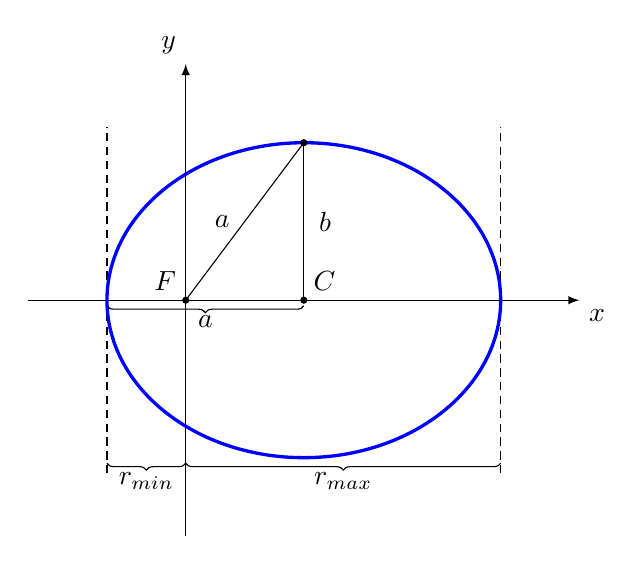
\begin{tikzpicture}
     \draw[-latex] (-2,0) -- (5,0) node[below right] {$x$};
     \draw[-latex] (0,-3) -- (0,3) node[above left] {$y$};
     \draw[densely dashed] (-1,-2.2) -- (-1,2.2);
     \draw[densely dashed] (4,-2.2) -- (4,2.2);
     \draw[blue,line width=1.2pt] (1.5,0) ellipse (2.5 and 2);
     \fill (1.5,0) circle (1.3 pt) node[above right] {$C$};
     \fill (0,0) circle (1.3 pt) node[above left] {$F$};
     \fill (1.5,2) circle (1.3 pt);
     \draw[decorate,decoration={brace,raise=2pt,mirror}] (-1,0) -- node[below=2pt]{$a$} (1.5,0);
     \draw (1.5,2) -- node[right=2pt]{$b$} (1.5,0);
     \draw (0,0) -- node[left=2pt]{$a$} (1.5,2);
     \draw[decorate,decoration={brace,mirror,raise=2pt}] (-1,-2) -- node[below=2pt]{$r_\text{min}$} (0,-2);
     \draw[decorate,decoration={brace,mirror,raise=2pt}] (0,-2) -- node[below=2pt]{$r_\text{max}$} (4,-2);
    \end{tikzpicture}
    \caption{A kapott ellipszispálya. A nagytengely hossza $a$ a kistengelyé $b$. Az origó az egyik fókusz ($F$), míg $C$ a centrum. Az origótól való legkisebb távolság $r_\text{min}$, a legnagyobb pedig $r_\text{max}$.}\label{fig:A13-ellipszis}
   \end{figure}
   Forgassuk el a koordináta-rendszert, hogy $\beta=0$ legyen. A legnagyobb és a legkisebb távolság, illetve a nagytengely hossza:
   \al{
    &r_\text{max}=\frac{p}{1-e}
    &r_\text{min}=\frac{p}{1+e}
    &&a=\frac{r_\text{max}+r_\text{min}}{2}
       =\frac{p}{1-e^2}.
   }
   A fókusz centrumtól mért távolsága, és a kistengely hossza:
   \al{
    &a-r_\text{min}=\frac{ep}{1-e^2}=e\cdot a.
    &b=\sqrt{a^2-(e\cdot a)^2}=\sqrt{a^2(1-e^2)}=\sqrt{a\cdot p},
   }
   amellyel a terület:
   \al{
    A=\pi ab =\pi\sqrt{a^3 p}.
   }
   A súrolt terület a területi sebesség és a periódusidő szorzataként is előáll (Kepler II{.}):
   \al{
    &\pi\sqrt{a^3 p}=T\cdot \frac{L}{2m}
    &\frac{T^2}{a^3}
      =\frac{4m^2\pi^2}{L^2}p
      =\frac{4m^2\pi^2}{L^2}\frac{L^2}{m\alpha}
      =\frac{4m\pi^2}{\alpha}
      =\text{állandó}.
   }
   Ez Kepler III.\ törvénye. Bolygómozgásnál $\alpha=mM\gamma$, így ott $\frac{T^2}{a^3}=\frac{4\pi^2}{M\gamma}$. A keringési idő bolygómozgásra:
   \al{
    T
    &=\sqrt{a^3\frac{4\pi^2}{M\gamma}}
     =\sqrt{\left(\frac{p}{1-e^2}\right)^3\frac{4\pi^2}{M\gamma}}
     =\sqrt{\left(\frac{\frac{L^2}{\gamma m^2 M}}{\frac{2\abs{E}L^2}{m\gamma^2 m^2 M^2}}\right)^3\frac{4\pi^2}{M\gamma}}
     =\sqrt{\left(\frac{m\gamma M}{2\abs{E}}\right)^3\frac{4\pi^2}{M\gamma}}\\
    &=\pi \gamma mM \sqrt{\frac{m}{2\abs{E}^3}}.
   }
 
 \section{Elektrodinamika} 
  
  \subsection{Coulomb-törvény kapcsolata a Maxwell-egyenletekkel}
   
   Lásd \ref{ss:01-CoulombMaxwell}. fejezet.
   
  \subsection{Oszcilláló töltéseloszlás tere}\label{ss:13-oszcillaloter}
   
   Tekintsünk olyan rendszert, ahol a potenciálok lokalizáltak (kiterjedése $d$), és szinuszosak: $\psi(\omega,\rv)$, $\Av(\omega,\rv)\sim e^{-i\omega t}$. Lorentz-mértékben: $0=\divo{\Av}+\frac{1}{c^2}\partial_t\phi=\divo{\Av}-\frac{1}{c^2}i\omega\phi$ így elég csak $\Av$-t kiszámítani, abból $\phi$ adódik.
   
   A retardált potenciálok (\ref{ss:9-retpot}. fejezet, illetve \eqref{eq:09-retpotA} egyenlet) szerint:
   \al{
    \vect{A}(t,\rv)
      &=\frac{\mu_0}{4\pi}\intl{}{}\dd^3\rv'\,\frac{\vect{J}\left(t-\frac{\abs{\rv-\rv'}}{c},\rv'\right)}{\abs{\rv-\rv'}}
       =\frac{\mu_0}{4\pi}\intl{}{}\dd^3\rv'\,\frac{\vect{J}(\rv')e^{-i\omega\left(t-\frac{\abs{\rv-\rv'}}{c}\right)}}{\abs{\rv-\rv'}}\\
    \vect{A}(\omega,\rv)
      &=\frac{\mu_0}{4\pi}\intl{}{}\dd^3\rv'\,\frac{\vect{J}(\rv')e^{ik\abs{\rv-\rv'}}}{\abs{\rv-\rv'}}
   }
   
   Közeltérben ($d\ll r\ll\lambda$), ahol $k\abs{\rv-\rv'}\ll 1$, nem számít a retardálás. A hullámzónában ($d\ll\lambda\ll r $) csak az $\sim\frac{1}{r}$ tagokat tartjuk meg:
   \al{
    \frac{1}{\abs{\rv-\rv'}}&=\frac{1}{r}+\mathcal{O}\left(\frac{d}{r^2}\right),\\
    \abs{\rv-\rv'}
      &=\sqrt{\rv^2-2\rv\rv'+\rv'^2}
      =r\sqrt{1-2\frac{\rv\rv'}{r^2}+\frac{\rv'^2}{\rv^2}}
      =r\sqrt{1-2\frac{\rv\rv'}{r^2}}+\mathcal{O}\left(\frac{d^2}{r}\right)\\
      &=r\left(1-\frac{\rv\rv'}{r^2}\right)+\mathcal{O}\left(\frac{d^2}{r}\right)
       =r-\rv'\ev_\rv+\mathcal{O}\left(\frac{d^2}{r}\right)\\
    e^{ik\abs{\rv-\rv'}}
      &\approx e^{ik(r-\rv'\ev_\rv)}
       =e^{ikr}e^{-ik\rv'\ev_\rv}
       \approx
        e^{ikr}\left(1-ik\rv'\ev_\rv\right),
   }
   az utolsó tagban felhasználtuk, hogy $k\abs{\rv'}<kd\ll 1$
   Így
   \aln{
    \vect{A}(\omega,\rv)
      &=\frac{\mu_0}{4\pi}\frac{e^{ikr}}{r}\intl{}{}\dd^3\rv'\,\vect{J}(\rv')\big(1-ik\rv'\ev_\rv\big)\label{eq:13-vectpot}
   }
    
   \paragraph{Mozgó töltés sugárzása}\label{ss:14-mogotoltessugarzasa}
    
    Tekintsünk egy ponttöltés, amely  általános mozgást végez: $\Jv(\rv)=q\vv(t)\delta\big(\rv-\vects{\gamma}(t)\big)$, ahol $\vects{\gamma}(t)$ a pálya. $\frac{1}{r}$-ed rendben \eqaref{eq:09-retpotA} egyenlet kiintegrálható:
    \al{
     \vect{A}(t,\rv)
      &\approx\frac{\mu_0}{4\pi}\intl{}{}\dd^3\rv'\,\frac{1}{r}q\vv(t)\delta\big(\rv'-\vects{\gamma}(t)\big)
       =\frac{\mu_0}{4\pi r}q\vv\left(t-\frac{r}{c}\right).
    }
    A deriválásnál is csak $\frac{1}{r}$-ed rendig tartjuk meg a tagokat, így $\vects{\nabla}\to-\frac{1}{c}\grad{r}\partial_t=-\frac{\rv}{rc}\partial_t=-\frac{\ev_\rv}{c}\partial_t$. A terek:
    \al{
     \Bv
      &=\rot{\Av}
       =\frac{q\mu_0}{4\pi}\rot{\vv\left(t-\frac{r}{c}\right)}
       =-\frac{q\mu_0}{4\pi c}\ev_\rv\times\partial_t\vv\left(t-\frac{r}{c}\right)
       =\frac{q\mu_0}{4\pi r c}\left[\av\left(t-\frac{r}{c}\right)\times\ev_\rv\right]  \\
     \dot{\Ev}
      &=c^2\rot{\Bv}
       =c^2\frac{q\mu_0}{4\pi r^2 c^2}\left[\dot{\av}\left(t-\frac{r}{c}\right)\times\ev_\rv\right]\times\ev_\rv\\
     \Ev
      &=\frac{q\mu_0}{4\pi r^2 }\left[\av\left(t-\frac{r}{c}\right)\times\ev_\rv\right]\times\ev_\rv
       =Z_0\Hv\times\ev_\rv.
    }
    A kisugárzott teljesítménysűrűség:
    \al{
     \Sv
      &=\Ev\times\Hv
       =Z_0(\Hv\times\ev_\rv)\times\Hv
       =Z_0\Hv^2\ev_\rv
       =Z_0\frac{q^2}{16\pi^2 r^2 c^2}\left[a\left(t-\frac{r}{c}\right)\right]^2\sin^2\vartheta\ev_\rv,
    }
    ahol $Z_0=\mu_0 c$ a vákuum ellenállása. Innen
    \aln{
     &\der{P}{\Omega}=\frac{Z_0 q^2}{16\pi^2 c^2}\left[a\left(t-\frac{r}{c}\right)\right]^2\sin^2\vartheta,
     &P=\frac{Z_0 q^2}{6\pi c^2}\left[a\left(t-\frac{r}{c}\right)\right]^2.\label{eq:13-Larmor}
    }
    Ez a Larmor-képlet. Látjuk, hogy a gyorsuló töltés sugároz. A képlet akkor használható, ha $d\ll \lambda\Leftrightarrow \frac{d}{\delta t}\ll \frac{\lambda}{\delta t}\Leftrightarrow v\ll c$, vagyis a nem relativisztikus határesetben.
    
    Körmozgásra $a\left(t-\frac{r}{c}\right)=\frac{v^2}{R}$:
    \al{
     P=\frac{Z_0 q^2}{6\pi c^2}\frac{v^4}{R^2}
      =\frac{Z_0 q^2 c^2}{6\pi R^2}\left(\frac{v}{c}\right)^4.
    }
    
   \paragraph{Sugárzás relativisztikus tárgyalása, Ciklotron sugárzás} 
    
    A relativisztikus tárgyaláshoz a Larmor-képletet relativisztikusan invariáns alakban kell felírni.
     
    A bal oldalon a teljesítmény $P=\der{E}{t}$, melyhez álló rendszerben $c\minv{p}^\mu=(E,0)$, és $\minv{x}^\mu=(ct,0)$. Mozgó rendszerbe való áttérésnél: $E\to E'=\frac{E}{\sqrt{1-v^2/c^2}}$ és $t\to t'=\frac{t}{\sqrt{1-v^2/c^2}}$, ahonnan: $\det{E}{t}=\der{E'}{t'}$, vagyis invariáns. 
    
    A jobb oldalon $\vect{a}$ nem kovariáns. A $v\to 0$ limesz ismeretében azzá tehetjük:
    \al{
     \minv{a}^\mu
      &=\der{^2\minv{r}^\mu}{^2\tau}
       =\der{}{\tau}\left(\frac{c}{\sqrt{1-\frac{v^2}{c^2}}},\frac{\vv}{\sqrt{1-\frac{v^2}{c^2}}}\right)
       =\frac{1}{\sqrt{1-\frac{v^2}{c^2}}^2}\left(0,\av\right)
        +\left(c,\vv\right)\der{}{\tau}\frac{1}{\sqrt{1-\frac{v^2}{c^2}}}\\
      &=\frac{1}{\sqrt{1-\frac{v^2}{c^2}}^2}\left(0,\av\right)
        +\frac{\vv\av}{c^2}\frac{1}{\sqrt{1-\frac{v^2}{c^2}}^4}\left(c,\vv\right)
       =\left(\frac{\vects{\beta}\av}{\sqrt{1-\frac{v^2}{c^2}}^4},\frac{\av}{\sqrt{1-\frac{v^2}{c^2}}^2}+\frac{(\vects{\beta}\av)\vects{\beta}}{\sqrt{1-\frac{v^2}{c^2}}^4}\right)\\
      &=\big(\gamma^4\vects{\beta}\av,\gamma^2\av+(\vects{\beta}\av)\vects{\beta}\gamma^4\big),
    }
    ami tudja, hogy $\minv{a}^\mu\to (0,\av)$, illetve $\minv{a}^\mu \minv{a}_\mu\to -\av^2$. Ezzel a Larmor-képlet felírva:
    \al{
     P=-\frac{Z_0 q^2}{6\pi c^2}\minv{a}^\mu \minv{a}_\mu,
    }
    szembeötlően invariáns. Visszaírjuk a gyorsulást és a sebességet:
    \al{
     \minv{a}^\mu\minv{a}_\mu
     &=\gamma^8(\vects{\beta}\av)^2-\gamma^4\av^2-(\vects{\beta}\av)^2\vects{\beta}^2\gamma^8-2\gamma^6(\vects{\beta}\av)^2\\
     &=-\gamma^4\av^2-\gamma^6(\vects{\beta}\av)^2+\gamma^6(\vects{\beta}\av)^2\Big[\underbrace{\gamma^2\big(1-\vects{\beta}^2\big)}_{=1}-1\Big]
      =-\gamma^4\av^2-\gamma^6(\vects{\beta}\av)^2.
    }
    Ez $\vv\to 0$-ra, visszaadja $-\av^2$-et, így a fenti kifejezés megfelel a klasszikus határesetnek. Alakítsuk még egy kicsit:
    \al{
     \minv{a}^\mu\minv{a}_\mu
      &=-\gamma^4\av^2-\gamma^6(\vects{\beta}\av)^2
       =-\gamma^6\big[(1-\betav^2)\av^2+(\vects{\beta}\av)^2\big]
       =-\gamma^6\big[\av^2+(\vects{\beta}\av)^2-\av^2\betav^2\big]\\
      &=-\gamma^6\big[\av^2+(\vects{\beta}\times\av)^2\big].
    }
    Ezzel tehát a Larmor-formula relativisztikus megfelelője:
    \al{
     P=\frac{Z_0 q^2}{6\pi c^2}\gamma^6\big[\av^2+(\vects{\beta}\times\av)^2\big].
    }
    Körmozgás esetén $\betav\perp\av$, így $(\vects{\beta}\times\av)^2=a^2\beta^2$, vagyis:
    \al{
     P=\frac{Z_0 q^2}{6\pi c^2}\gamma^6\big[(1-\beta^2)a^2\big]
      =\frac{Z_0 q^2}{6\pi c^2}\gamma^4 a^2.
    }
    A klasszikus képletet képest ez egy $\gamma^4$-es faktorban tér el. Ha $v\sim c$, akkor a sugárzás teljesítménye nagyon megnő.
    
    
 \section{Kvantummechanika}
  
  \subsection{Kötött állapot} 
   
   Kötött állapotról akkor beszélünk, ha a rendszer spektruma pontspektrum. Ekkor a hullámfüggvény normálható, és az eleme a négyzetesen integrálható függvények Hilbert-terének.
   
  \subsection{Schrödigner-egyenlet centrális erőtérben}
   
   Legyen a potenciál centrális, azaz $\opV(\oprv)=\opV(\opr)$. Ekkor a Schrödinger-egyenlet gombi koordinátákban, koordinátareprezentációban:
   \al{
    \left\{-\frac{\hbar^2}{2m}\left[\frac{1}{r}\partial_r^2r+\frac{1}{r^2}\left(\partial_{\vartheta}+\frac{1}{\tg{\vartheta}}\partial_{\vartheta}^2+\frac{1}{\sin^2{\varphi}}\partial_{\vartheta}^2\right)\right]+V(r)\right\}\psi(r,\vartheta,\varphi)=E\psi(r,\vartheta,\varphi).
   }
   Az 
   \al{
    L^2=-\hbar^2\left(\partial_{\vartheta}^2+\frac{1}{\tg{\vartheta}}\partial_{\vartheta}+\frac{1}{\sin^2{\vartheta}}\partial_{\varphi}^2\right)
   }
   sajátérték problémájának megoldását lásd \ref{ss:06-L2spme}. fejezet. A megoldást akkor keressük
   \al{
    \psi(r,\vartheta,\varphi)=\frac{1}{r}R(r)Y_l^m(\vartheta,\varphi)
   }
   alakban, melyet behelyettesítve az egyenletbe a radiális Schrödinger-egyenletet kapjuk:
   \aln{
    \left[-\frac{\hbar^2}{2m}\frac{1}{r}\partial_r^2r+\frac{\hbar^2 l(l+1)}{2mr^2}+V(r)\right]\psi(r,\vartheta,\varphi)&=E\psi(r,\vartheta,\varphi)\nonumber\\
    \left[-\frac{\hbar^2}{2m}\der{^2}{r^2}+\frac{\hbar^2 l(l+1)}{2mr^2}+V(r)\right]R(r)&=ER(r).\label{eq:13:radSch}
   }
   
  \subsection{Hidrogénatom}
   
   Legyen $V(r)=-\frac{kZe^2}{r}$. Az állapotok negatív energiájúak: $E=-\abs{E}$. Ezzel az egyenlet:
   \al{
    0=\left[-\frac{\hbar^2}{2m}\der{^2}{r^2}+\frac{\hbar^2 l(l+1)}{2mr^2}-\frac{kZe^2}{r}+\abs{E}\right]R(r).
   }
   Bevzetjük az alábbi jelöléseket:
   \al{
    &r_0=\frac{\hbar}{\sqrt{2m\abs{E}}}
    &\xi=\frac{\sqrt{8m\abs{E}}}{\hbar}r=\frac{2r}{r_0}
    &&a_0=\frac{\hbar^2}{mke^2}
    &&\ep=\frac{Zke^2\sqrt{2m\abs{e}}}{2\hbar\abs{E}},
   }
   melyekkel
   \al{
    \der{^2R(\xi)}{\xi^2}+\left[-\frac{1}{4}+\frac{\ep}{\xi}-\frac{l(l+1)}{\xi^2}\right]R(\xi)=0.
   }
   
   \paragraph{Sommerfeld polinommódszer}
    
    Először megkeressük az aszimptotikus megoldást:
    \al{
     &\xi\to 0
     &\der{^2R(\xi)}{\xi^2}-\frac{l(l+1)}{\xi^2}R(\xi)=0
     &&R(\xi)\sim\xi^{l+1},\\
     &\xi\to \infty
     &\der{^2R(\xi)}{\xi^2}-\frac{1}{4}R(\xi)=0
     &&R(\xi)\sim e^{-\frac{1}{2}\xi}.
    }
    
    A megoldást keressük egy polinom és az aszimptotikus megoldás szorzataként: $R(\xi)=u(\xi)e^{-\frac{1}{2}\xi}$, mellyel
    \al{
     &\dd_\xi R(\xi)=\left(-\frac{1}{2}u(\xi)+u'(\xi)\right)e^{-\frac{1}{2}\xi}
     &\dd_\xi^2 R(\xi)=\left(\frac{1}{4}u(\xi)-u'(\xi)+u''(\xi)\right)e^{-\frac{1}{2}\xi},
    }
    így
    \al{
     u''(\xi)-u'(\xi)+\left[\frac{\ep}{\xi}-\frac{l(l+1)}{\xi^2}\right]u(\xi)=0.
    }
    A hatványsor legyen $u(\xi)=\xi^s\suml{i=0}{\infty}c_i\xi^i$, ahol $s$ az iniciális index. Ennek deriváltjai:
    \al{
     u'(\xi)&=\suml{i=0}{\infty}(i+s)c_i\xi^{i+s-1}
      =\suml{i=1}{\infty}(i+s-1)c_{i-1}\xi^{i+s-2}\\
     u''(\xi)&=\suml{i=0}{\infty}(i+s)(i+s-1)c_i\xi^{i+s-2},
    }
    majd behelyettesítve:
    \al{
     0
      &=\suml{i=0}{\infty}(i+s)(i+s-1)c_i\xi^{i+s-2}-\suml{i=1}{\infty}(i+s-1)c_{i-1}\xi^{i+s-2}+\left[\frac{\ep}{\xi}-\frac{l(l+1)}{\xi^2}\right]\suml{i=0}{\infty}c_{i}\xi^{i+s}\\
      &=s(s-1)c_0\xi^{s-2}+\suml{i=1}{\infty}\bigg(
       (i+s)(i+s-1)c_i\xi^{i+s-2}
      -(i+s-1)c_{i-1}\xi^{i+s-2}\bigg)\\
      &\qquad\qquad\qquad+\suml{i=0}{\infty}\left[\ep c_{i}\xi^{i+s-1}-l(l+1)c_{i}\xi^{i+s-2}\right]\\
      &=\big[s(s-1)-l(l+1)\big]c_0\xi^{s-2}+\suml{i=1}{\infty}\bigg(
        \big[(i+s)(i+s-1)-l(l+1)\big]c_i\\
      &\qquad\qquad\qquad\qquad\qquad\qquad\qquad\qquad\qquad\qquad\qquad\qquad
        +\big[\ep-(i+s-1)\big]c_{i-1}\bigg)\xi^{i+s-2}.
    }
    Ennek mindegyik együtthatója el kell, hogy tűnjön. $c_0\ne 0$, mert biztos van egy olyan $c_i$, így $s=l+1$ vagy $s=-l$, ahonnan csak az első jön szóba, a $\xi\to 0$-ban való regularitás miatt. A többi együtthatóra:
    \al{
     c_i
      =\frac{-\ep+(i+s-1)}{(i+s)(i+s-1)-l(l+1)}c_{i-1}
      =\frac{-\ep+i+l}{i(i+2l+1)}c_{i-1}.
    }
    Nagy $i$-re $\frac{c_i}{c_{i-1}}\sim\frac{1}{i}$, ami így azt eredményezné, hogy $u\sim e^{\xi}$, vagyis $R(\xi)\sim e^{\frac{1}{2}\xi}$, ami nem reguláris. Emiatt léteznie kell egy $i_\text{max}$-nak, hogy $c_{i_\text{max}}=0$. Ekkor 
    \al{
     i_\text{max}+l-\ep=0.
    }
    Bevezetjük az
    \al{
     n=i_\text{max}+l=\ep,
    }
    főkvantumszámot, ami: $n>l$, $n=1,2,3,\dots$, illetve $n=\frac{Z r_0}{a_0}$. Az eredmény összefoglalva:
    \al{
     E_n
      &=-\frac{\hbar^2}{2m r_0^2}
       =-\frac{Z^2\hbar^2}{2m a_0^2}\frac{1}{n^2}
       =-\frac{mZ^2 k^2e^4}{2\hbar^2}\frac{1}{n^2}
       =-\frac{mZ^2e^4}{32\pi^2\ep_0^2\hbar^2}\frac{1}{n^2},
    }
    \al{
     \psi(r,\vartheta,\varphi)
      &=
       \sqrt{{\left (\frac{2}{r_0} \right ) }^3\frac{(n-l-1)!}{2n\,(n+l)!} } 
       \left(\frac{2r}{r_0}\right)^l L_{n-l-1}^{2l+1}\left(\frac{2r}{r_0}\right)e^{-\frac{r}{r_0}}Y_l^m(\vartheta,\varphi),
    }
    ahol $L_{n-l-1}^{2l+1}\left(\frac{2r}{r_0}\right)$ az asszociált Laguerre-polinomok:
    \al{
     L_n^{\alpha}(x)=\frac{x^{-\alpha} e^x}{ n!}\frac{d^n}{dx^n} \left(e^{-x} x^{n+\alpha}\right).
    }
    \begin{figure}[ht!]
     \centering
    \subfloat[$n=1$\label{fig:A13-e1}]{\includegraphics[width= 0.3\textwidth]{./A13tetel/H-n1}} \hspace{6pt}
    \subfloat[$n=2$\label{fig:A13-e2}]{\includegraphics[width= 0.3\textwidth]{./A13tetel/H-n2}} \hspace{6pt}
    \subfloat[$n=3$\label{fig:A13-e3}]{\includegraphics[width= 0.3\textwidth]{./A13tetel/H-n3}}
     \caption{Radiális valószínűségek ($w_{n,l}(r)=\abs{\Psi_r(r)}^2\cdot r^2$) az első három energiaszinthez tartozó hullámfüggvények esetében. (Az $y$ tengely skálája változik az ábrákon!)}
    \end{figure}
    
%     \al{
%      L_{n-l-1}^{2l+1}\left(\frac{r}{2r_0}\right)=\frac{\left(\frac{r}{2r_0}\right)^{-(2l+1)} e^{\frac{r}{2r_0}}}{ (n-l-1)!}\frac{\dd^{n-l-1}}{\dd \left(\frac{r}{2r_0}\right)^{n-l-1}} \left(e^{-\frac{r}{2r_0}} \left(\frac{r}{2r_0}\right)^{(n-l-1)+(2l+1)}\right).
%     }
    
    
    
    
    
